\documentclass[hidelinks,12pt]{article}
\usepackage[left=0.25cm,top=1cm,right=0.25cm,bottom=1cm]{geometry}
%\usepackage[landscape]{geometry}
\textwidth = 20cm
\hoffset = -1cm
\usepackage[utf8]{inputenc}
\usepackage[spanish,es-tabla]{babel}
\usepackage[autostyle,spanish=mexican]{csquotes}
\usepackage[tbtags]{amsmath}
\usepackage{nccmath}
\usepackage{amsthm}
\usepackage{amssymb}
\usepackage{mathrsfs}
\usepackage{graphicx}
\usepackage{subfig}
\usepackage{standalone}
\usepackage[outdir=./Imagenes/]{epstopdf}
\usepackage{siunitx}
\usepackage{physics}
\usepackage{color}
\usepackage{float}
\usepackage{hyperref}
\usepackage{multicol}
%\usepackage{milista}
\usepackage{anyfontsize}
\usepackage{anysize}
%\usepackage{enumerate}
\usepackage[shortlabels]{enumitem}
\usepackage{capt-of}
\usepackage{bm}
\usepackage{relsize}
\usepackage{placeins}
\usepackage{empheq}
\usepackage{cancel}
\usepackage{wrapfig}
\usepackage[flushleft]{threeparttable}
\usepackage{makecell}
\usepackage{fancyhdr}
\usepackage{tikz}
\usepackage{bigints}
\usepackage{scalerel}
\usepackage{pgfplots}
\usepackage{pdflscape}
\pgfplotsset{compat=1.16}
\spanishdecimal{.}
\renewcommand{\baselinestretch}{1.5} 
\renewcommand\labelenumii{\theenumi.{\arabic{enumii}})}
\newcommand{\ptilde}[1]{\ensuremath{{#1}^{\prime}}}
\newcommand{\stilde}[1]{\ensuremath{{#1}^{\prime \prime}}}
\newcommand{\ttilde}[1]{\ensuremath{{#1}^{\prime \prime \prime}}}
\newcommand{\ntilde}[2]{\ensuremath{{#1}^{(#2)}}}

\newtheorem{defi}{{\it Definición}}[section]
\newtheorem{teo}{{\it Teorema}}[section]
\newtheorem{ejemplo}{{\it Ejemplo}}[section]
\newtheorem{propiedad}{{\it Propiedad}}[section]
\newtheorem{lema}{{\it Lema}}[section]
\newtheorem{cor}{Corolario}
\newtheorem{ejer}{Ejercicio}[section]

\newlist{milista}{enumerate}{2}
\setlist[milista,1]{label=\arabic*)}
\setlist[milista,2]{label=\arabic{milistai}.\arabic*)}
\newlength{\depthofsumsign}
\setlength{\depthofsumsign}{\depthof{$\sum$}}
\newcommand{\nsum}[1][1.4]{% only for \displaystyle
    \mathop{%
        \raisebox
            {-#1\depthofsumsign+1\depthofsumsign}
            {\scalebox
                {#1}
                {$\displaystyle\sum$}%
            }
    }
}
\def\scaleint#1{\vcenter{\hbox{\scaleto[3ex]{\displaystyle\int}{#1}}}}
\def\bs{\mkern-12mu}


%\usepackage{showframe}
\usepackage{apacite}
\title{Funciones ordinarias de Laguerre \\ \large {Tema 5 - Funciones especiales} \vspace{-3ex}}
\author{M. en C. Gustavo Contreras Mayén}
\date{ }
\begin{document}
\vspace{-4cm}
\maketitle
\fontsize{14}{14}\selectfont
\tableofcontents
\newpage
%Referencia. Debnath - Integral transforms and their applications. Sec. 1.1
\section{Breve introducción.}
Las transformadas integrales se han utilizado con éxito durante casi dos siglos para resolver muchos problemas en matemática aplicada, física matemática y ciencias de la ingeniería.
\par
Históricamente, el origen de las transformaciones integrales, incluidas las transformadas de Laplace y de Fourier, se remonta a la célebre obra de Laplace (1749-1827) sobre la teoría de la probabilidad en la década de 1780 y al tratado monumental de Joseph Fourier (1768-1830) en \emph{La Théorie Analytique de la Chaleur} publicada en 1822. De hecho, el libro clásico de Laplace \emph{La Théorie Analytique des Probabilities} incluye algunos resultados básicos de la transformada de Laplace, que es una de las transformadas integrales más antiguas y más utilizadas en la literatura matemática. 
\par
Esto se ha utilizado efectivamente para encontrar la solución de ecuaciones diferenciales lineales y ecuaciones integrales. Por otro lado, el tratado de Fourier proporcionó la teoría matemática moderna de la conducción de calor, las series de Fourier y las integrales de Fourier con aplicaciones. En su tratado, Fourier declaró un resultado notable que se conoce universalmente como el \emph{Teorema Integral de Fourier}. Proporcionó una serie de ejemplos antes de afirmar que una función arbitraria definida en un intervalo finito puede expandirse en términos de series trigonométricas que ahora se conocen universalmente como la \emph{serie de Fourier}.
\par
En un intento por extender sus nuevas ideas a funciones definidas en un intervalo infinito, Fourier descubrió una transformada integral y su fórmula de inversión que ahora se conocen como la \emph{transformada de Fourier} y la \emph{transformada de Fourier inversa}. Sin embargo, esta célebre idea de Fourier era conocida por Laplace y Cauchy (1789–1857), ya que algunos de sus trabajos anteriores implicaban esta transformada. Por otro lado, Poisson (1781–1840) también utilizó de manera independiente el método de transformada en su investigación sobre la propagación de ondas de agua.
\par
Sin embargo, fue Leibniz (1646–1716) quien introdujo por primera vez la idea de un método simbólico en el cálculo. Posteriormente, tanto Lagrange (1736–1813) como Laplace hicieron contribuciones considerables a los métodos simbólicos que se conocieron como cálculo operacional. Aunque tanto la transformada de Laplace como la de Fourier se descubrieron en el siglo XIX, fue el ingeniero eléctrico británico Oliver Heaviside (1850–1925) quien hizo la transformada de Laplace muy popular al usarla para resolver ecuaciones diferenciales ordinarias de circuitos y sistemas eléctricos, y luego desarrollar el cálculo operacional moderno.
\par
Puede ser relevante señalar que la transformada de Laplace es esencialmente un caso especial de la transformada de Fourier para una clase de funciones definidas en el eje real positivo, pero es más simple que la transformada de Fourier por las siguientes razones.
\begin{enumerate}
\item La cuestión de la convergencia de la transformada de Laplace es mucho menos delicada debido al kernel de la exponencial decreciente $\exp (-s \, t)$, donde $\Re{s} > 0$ y $t > 0$.
\item La transformada de Laplace es una función analítica de variable compleja y sus propiedades pueden ser fácilmente estudiadas con el conocimiento de la teoría de la variable compleja.
\item La fórmula integral de Fourier proporcionó las definiciones de la transformada de Laplace y la transformada inversa de Laplace en términos de una integral de contorno complejo que se puede evaluar con la ayuda de la teoría del residuo de Cauchy y la deformación del contorno en el plano complejo.
\end{enumerate}

\section{Conceptos básicos y definiciones.}
La transformada integral de una función $f(x)$ definida en el intervalo $a \leq x \leq b$, se escribe como $\mathscr{I} \left\{ f(x) \right\} = F(x)$ y se define por
\begin{align}
\mathscr{I} \left\{ f(x) \right\} = F(k) = \int_{a}^{b} K(x, k) \, f(x) \dd{x}
\label{eq:ecuacion_01_02_01}
\end{align}
donde $K(x, k)$ es una función dada de dos variables $x$ y $k$, que se le llama \emph{kernel} de la transformada. El operador $\mathscr{I}$ es llamada \emph{operador de transformada integral} o simplemente \emph{transformada integral}.
\par
La función transformada $F(k)$ se refiera a menudo como la \emph{imagen} de la función dada $f(x)$, y $k$ es llamada la \emph{variable transformada}.
\par
De manera similar, la transformada integral de una función de varias variables se define por
\begin{align}
\mathscr{I} \left\{ f(x) \right\} = F(\mathbf{k}) = \int_{S} K(\mathbf{x}, \mathbf{k}) \, f(\mathbf{x}) \dd{x}
\label{eq:ecuacion_01_02_02}
\end{align}
donde $\mathbf{x} = (x_{1}, x_{2}, \ldots, x_{n}), \mathbf{k} = (k_{1}, k_{2}, \ldots, k_{n})$ y $S \in R^{n}$
%Referencia Arfken - Mathematical methods for physicists. Cap. 15 Integral Transforms -djvu
% \section{Transformadas Integrales.}
% Frecuentemente en física uno se encuentra con pares de funciones que se encuentran relacionadas por una expresión como la siguiente
% \begin{equation}
% g (\alpha) = \int_{a}^{b} f(t) \, K(\alpha, t) \, \dd t
% \label{eq:ecuacion_15_01}
% \end{equation}
% La función $g (\alpha)$ es llamada la transformada integral de $f(t)$ por el núcleo (o kernel)  $K (\alpha,t)$.
\par
La operación de transformación se puede describir como un mapeo de una función $f(t)$ en el espacio-$t$ a otra función $F (\alpha)$ en el espacio-$\alpha$. Dos ejemplos de esta interpretación en física son las relaciones entre: el tiempo y la frecuencia en Electrodinámica Clásica y Mecánica Cuántica, y la relación entre el espacio de configuraciones y el espacio de momentos en Mecánica Cuántica.
\par
Cuando los límites de integración $a$ y $b$ son finitos, decimos que $F(\alpha)$ es es la transformada finita de $f(x)$. 

\subsection{Las transformadas integrales.}

Existen varios tipos de transformadas integrales que aparecen frecuentemente en la física matemática, cada una de ellas está asociada a un kernel (núcleo) diferente. De entre las diferentes posibilidades podemos mencionar los núcleos siguientes:
\begin{enumerate}
\item \emph{Transformada de Fourier.}
\begin{align}
g (\omega) = \dfrac{1}{\sqrt{2 \, \pi}} \int_{-\infty}^{\infty} f(t) \, e^{i \omega t} \, \dd{t}
\label{eq:ecuacion_07_01}
\end{align}
\item \emph{Transformada de Laplace.}
\begin{align}
g (\alpha)= \int_{0}^{\infty} f(t) \; \exp(-\alpha t) \, \dd{t}
\label{eq:ecuacion_7_02}
\end{align}
\item \emph{Transformadas de Fourier seno y coseno.}
\begin{align}
g (\alpha)= \int_{0}^{\infty} f(t) \; \substack{ \textstyle \sin \\[0.5em] \textstyle \cos} \; \alpha \, t \,  \dd{t}
\label{eq:ecuacion_7_03}
\end{align}
\item \emph{Transformada de Fourier compleja.}
\begin{align}
g (\alpha)= \int_{-\infty}^{\infty} f(t) \; \exp(i \alpha t) \, \dd{t}
\label{eq:ecuacion_7_04}
\end{align}
\item \emph{Transformada de Hankel.}
\begin{align}
g (\alpha)= \int_{0}^{\infty} f(t) \; t \; J_{n} (\alpha \, t) \, \dd{t}
\label{eq:ecuacion_7_05}
\end{align}
donde $J_{n}(\alpha t)$ es la función de Bessel de primera clase de orden $n$.
\item \emph{Transformada de Mellin.}
\begin{align}
g (\alpha)= \int_{0}^{\infty} f(t) \; t^{\alpha-1} \, \dd{t}
\label{eq:ecuacion_7_06}
\end{align}
%Ref. Debnath (2007) 
\item \emph{Transformada de Hilbert.}
\begin{align}
\mathbf{H} \left\{ f(t) \right\} = \hat{f}_{\mathbf{H}} (x) = \dfrac{1}{\pi} \oint_{\infty}^{\infty} \dfrac{f(t)}{t - x} \dd{t}
\label{eq:ecuacion_9_2_1}
\end{align}
\item \emph{Transformada de Stieltjes.}
\begin{align}
\mathscr{I} \left\{ f(t) \right\} = \tilde{f} (z) = \int_{0}^{\infty} \dfrac{f(t)}{t + z} \dd{t}
\label{eq:ecuacion_9_7_2}
\end{align}
\item \emph{La transformada Z.}
\begin{align}
\mathscr{L} \left\{ f^{*} (t) \right\} = F(z) = \sum_{n=0}^{\infty} f( n\, T) \, \exp(- n \, s \, T)
\label{eq:ecuacion_12_3_1}
\end{align}
\item \emph{Transformada de Legendre.}
\begin{align}
\mathscr{T} \left\{ f(x) \right\} = \tilde{f} (n) = \int_{-1}^{1} P_{n} \, f(x) \dd{x}
\label{eq:ecuacion_14_2_1}
\end{align}
donde $P_{n}(x)$ es el polinomio de Legendre de grado n $(\geq 0)$.
\item \emph{Transformada de Jacobi.}
\begin{align}
J \left\{ F(x) \right\} = f^{(\alpha, \beta)} \, (n) = \int_{-1}^{1} (1 - x)^{\alpha} \, (1 + x)^{\beta} \, P_{n}^{(\alpha, \beta)} \, (x) \, F(x) \dd{x}
\label{eq:ecuacion_15_2_1}
\end{align}
donde $P_{n}^{(\alpha, \beta)} \, (x)$ es el polinomio de Jacobi de orden $n$ y ordenes $\alpha (> -1)$ y $\beta (> -1)$.
\item Cuando $\alpha = \beta = \nu - 1/2$, la transformada de Jacobi (ec. \ref{eq:ecuacion_15_2_1}), se reduce a la \emph{Transformada de Gegenbauer}:
\begin{align}
G \left\{ F(x) \right\} = f^{(\nu)} \, (n) = \int_{-1}^{1} (1 - x^{2})^{\nu - 1/2} \, C_{n}^{\nu} \, (x) \, F(x) \dd{x}
\label{eq:ecuacion_15_2_4}
\end{align}
\item \emph{Transformada de Laguerre.}
\begin{align}
L \left\{ f(x) \right\} = \tilde{f}_{\alpha} (n) = \int_{0}^{\infty} e^{-x} \, x^{\alpha} \, L_{n}^{\alpha} \, (x) \, f(x) \dd{x}
\label{eq:ecuacion_16_2_1}
\end{align}
donde $L_{n}^{\alpha} \, (x)$ es el polinomio asociado de Laguerre de orden $n (\leq 0)$ y orden $\alpha (> 1)$.
\item \emph{Transformada de Hermite.}
\begin{align}
H \left\{ F(x) \right\} = f_{H} (n) = \int_{-\infty}^{\infty} \exp(-x^{2}) \, H_{n} (x) \, F(x) \dd{x}
\label{eq:ecuacion_17_2_1}
\end{align}
donde $H_{n}$ es el polinomio de Hermite de grado $n$.
\item \emph{Transformada de Radon.}
Si $L$ es cualquier línea recta en el plano $x-y$ (o, en $\mathbb{R}^{2}$) y $\dd{s}$ es la longitud del arco a lo largo de $L$ (ver la figura \ref{eq:figura_Radon})
\begin{figure}[H]
    \centering
    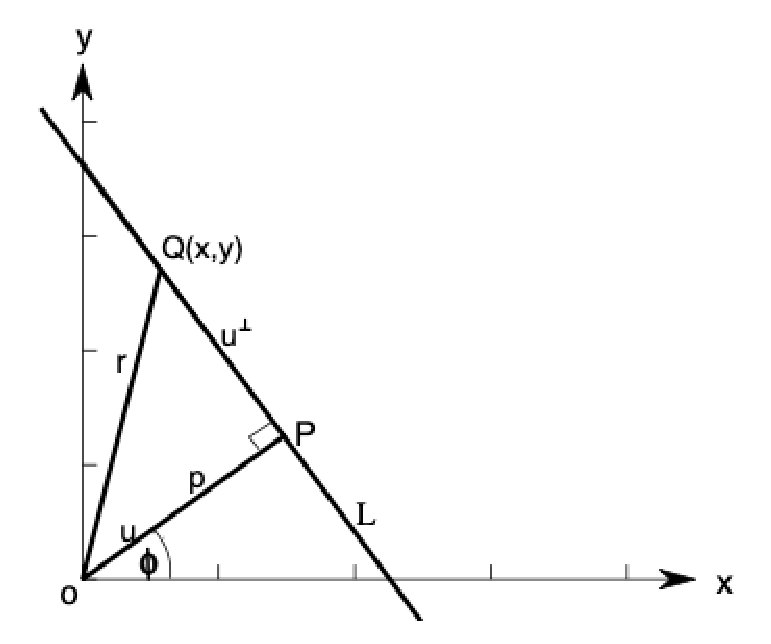
\includegraphics[scale=0.7]{Imagenes/Transformada_Radon_01.eps}
    \caption{Descripción de la línea recta para la definición de la trasformada de Radon.}
    \label{eq:figura_Radon}
\end{figure}
La transformada de Radon de una función $f (x, y)$ de dos variables reales se define por su integral a lo largo de $L$ como:
\begin{align}
\hat{f} (p, \phi) = \mathscr{R} \left\{ f(x, y) \right\} = \int_{L} f(x, y) \dd{s}
\label{eq:ecuacion_18_2_1}
\end{align}
\item \emph{Transformada Wavelet.}
La transformada Wavelet continua\footnote{Traducir al español como tal el término wavelet, nos dejaría alguna de las siguientes opciones: \emph{ondícula, onduleta u onditas}; siendo claro que en estos casos no es conveniente traducir, ya que al dejar el término en inglés, se mantiene la idea principal, mientras que en español, queda descontextualizado.} es similar a la transformada de Fourier en el sentido de que se basa en una sola función $\psi$ y que esta función está escalada. Pero a diferencia de la transformada de Fourier, también cambiamos la función, generando así una familia de funciones de dos parámetros $\psi_{a, b}$. Es conveniente definir $\psi_{a, b}$ como sigue:
\begin{align*}
\psi_{a, b} (x) = \abs{a}^{1/2} \, \psi \left( \dfrac{x - b}{a} \right)
\end{align*}
Entonces la \emph{transformada Wavelet continua} se define por:
\begin{align*}
(W_{\psi} \, f) (a, b) = \int_{-\infty}^{\infty} f(t) \, \overline{\psi_{a, b} (t)} \dd{t} = \abs{a}^{1/2} \, \int_{-\infty}^{\infty} f(t) \, \overline{\psi \left( \dfrac{x - b}{a} \right)} \dd{t}
\end{align*}
\end{enumerate}
Para cada una de la tranformadas integrales listadas, se debe de considerar su correspondiente transformada inversa.

\subsection{¿Por qué usar transformadas?}

Como se verá más adelante, aplicar una transformada integral a una EDP es para excluir temporalmente una variable independiente que se ha elegido y dejar de solución de una EDP en una variable menos. La solución de esta ecuación será una función de $\alpha$ y las variables restantes. Cuando se ha obtenido esta solución, tiene que ser \enquote{invertida} para recuperar la variable \enquote{perdida}: Así, si $t$ es la variable eliminada y $g (\alpha)$ es una de las transformaciones dadas anteriormente, obtenemos primero las ecuaciones auxiliares que dan $g$ en términos de $\alpha$ y las variables independientes restantes, resolvemos para $g$ y luego inviertimos para obtener $g(\alpha)$.
\par
El proceso de inversión significa, en efecto, la solución de una de las ecuaciones integrales (\ref{eq:ecuacion_7_02}) $\ldots$ (\ref{eq:ecuacion_7_06}), $g (\alpha)$ que se supone conocido y $f(t)$ que se encuentran, como se puede ver en la figura (\ref{fig:figura_01}). Tales soluciones son conocidas y pueden ser obtenidos formalmente del teorema de la integral de Fourier.
\begin{figure}[H]
    \centering
    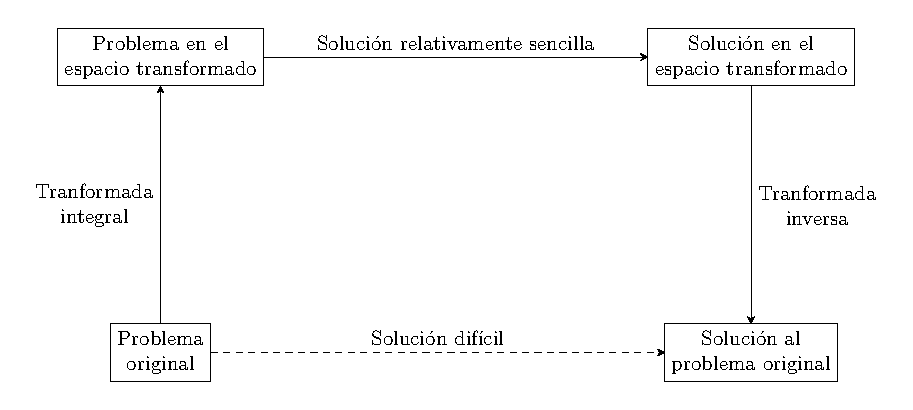
\includegraphics[scale=1]{Imagenes/esquema_transformadas.eps}
    \caption{Esquema de las transformadas integrales.}
    \label{fig:figura_01}
\end{figure}
\subsection{Linealidad de las transformadas integrales.}
Todas estas transformadas integrales son lineales, por lo que satisfacen las siguientes propiedades:
\begin{align}
\begin{aligned}
\int_{a}^{b} [ c_{1} \, f_{1} (t) + c_{2} \, f_{2}(t)] \; K(\alpha, t) \, \dd{t} &= c_{1} \, \int_{a}^{b} f_{1} (t) \; K(\alpha, t) \, \dd{t} + \\
&+ c_{2} \, \int_{a}^{b} f_{2} (t) \; K(\alpha, t) \, \dd{t}
\end{aligned}
\label{eq:ecuacion_15_08} 
\end{align}
y además
\begin{align}
\int_{a}^{b}  c \; f (t) \; K(\alpha, t) \, \dd t =  c \; \int_{a}^{b} f (t) \; K(\alpha, t) \, \dd{t}
\label{eq:ecuacion_15_09}
\end{align}
donde $c_{1}$ y $c_{2}$ son constantes y $f_{1}(t)$ y $f_{2}(t)$ son funciones para las cuales la operación transformada está definda.
\par
Representando la transformada integral lineal por el operador $\mathcal{L}$, obtenemos
\begin{align}
g (\alpha) = \mathcal{L} \, f(t)
\label{eq:ecuacion_15_10}
\end{align}
Uno espera que exista el operador inverso $\mathcal{L}^{-1}$, de manera tal que
\begin{align}
f(t) = \mathcal{L}^{-1}  \; g (\alpha)
\label{eq:ecuacion_15_11}
\end{align}
En general, el mayor problema con el uso de las transformadas integrales, es determinar el operador inverso. Sin embargo, para los dos tipos de transformaciones: de Fourier y de Laplace, obtener el inverso es relativamente sencillo.

%Ref. Patra (2018) 1.2 Classes of functions.
\section{Tipos de funciones.}

Una función de valor único $f (x)$ de la variable independiente $x$ que es continua en un intervalo $[a, b]$, se dice que pertenece a una clase denotada por $f \in C \, [a, b]$.
\par
Se dice que una función $f (x)$ es continua por partes en un intervalo $(a, b)$ si el intervalo se puede dividir en un número finito de subintervalos que no se intersecan $(a, a_{1}), (a_{1}, a_{2}), \ldots, (a_{n -1}, b)$, en cada uno de los cuales la función es continua y tiene límites finitos cuando $x$ se acerca a los puntos extremos de cada uno de los subintervalos. Se dice que dicha función pertenece a una clase denotada por $f \in P \, (a, b)$.
\par
Una función continua a trozos $f$ en $(a, b)$, cuya derivada de primer orden es también una función continua a trozos en $(a, b)$ y pertenece a una clase denotada por $f \in P^{1} \, (a, b)$.
\par
Se dice que el conjunto de funciones $f (x)$ es absolutamente integrable sobre $\Omega$, si $\int_{\Omega}  \abs{f (x)} \dd{x}$ es finito. Entonces decimos que esta función pertenece a una clase denotada por $f (x) \in A_{1} (\Omega)$. De manera similar, el hecho que $f \in A_{m} (\Omega)$ implica que $\int_{\Omega}  \abs{f (x)} \dd{x}$ es finito.
\par
Finalmente, presentamos una clase de funciones $f (x)$, que satisface las siguientes condiciones:
\begin{enumerate}[label=\roman*]
\item $f (x)$ se define en $c < x < c + 2 \, l$.
\item $f (x)$ es una función periódica del período $2 \, l$.
\item $f (x)$ y $\ptilde{f} (x)$ son continuas por partes en $c  < x <c + 2 \, l$ expresado por $f (x) \in P^{1} (c, c + 2 \, l)$.
\end{enumerate}
Se dice que esta clase de función $f (x)$ satisface las condiciones de Dirichlet. Se dice que una función $f (x)$ es de orden exponencial $\sigma$ cuando $x \to \infty$, si las constantes $\sigma, m (> 0)$ se pueden encontrar de modo que:
\begin{align*}
\abs{ e^{\sigma \, x} \, f(x)} < m \hspace{1cm} \Longrightarrow \hspace{1cm} \abs{f(x)} < m \, e^{m \, \sigma} \hspace{0.5cm} x > x_{0}
\end{align*}
De manera equivalente, también se puede escribir $f (x) = 0 \, (e^{m \, \sigma})$ mientras $x \to \infty$.

%Ref. Patra (2018) 1.3 Series de Fourier y la Fórmula Integral de Fourier.

\section{Series de Fourier y la fórmula integral de Fourier.}

Consideremos una función $f(x)$ que satisface las condiciones de Dirichlet en el intervalo $[-l, l]$, la función pertenece a la clase $P^{1} (R)$ y también a la clase $A_{1} (R)$. Sea el período principal de $f(x)$ igual a $2 \, l$. Entonces $f(x)$ admite una representación en una serie de Fourier:
\begin{align*}
f(x) = a_{0} + \sum_{n=1}^{\infty} \left[ a_{n} \, \cos \left( \dfrac{n \, \pi, \, x}{l}  \right) + b_{n} \, \sin \left( \dfrac{n \, \pi, \, x}{l}  \right) \right]
\end{align*}
donde:
\begin{align*}
a_{0} &= \dfrac{1}{2 \, l} \int_{-l}^{l} f(x) \dd{x} \\[0.5em]
(a_{n}, b_{n}) &= \dfrac{1}{l} \int_{-l}^{l} f(x) \left[ \cos \left( \dfrac{n \, \pi \, x}{l} \right), \sin \left( \dfrac{n \, \pi \, x}{l} \right) \right] \dd{x}
\end{align*}
entonces:
\begin{align*}
a_{n} - i \, b_{n} = \dfrac{1}{l} \int_{-l}^{l} f(x) \, \exp \left( - \dfrac{i \, n \, \pi \, x}{l} \right) \dd{x}
\end{align*}
Definimos a continuación:
\begin{align*}
a_{0} &= c_{0} \\
a_{n} &= c_{n} + c_{-n} \\
i \, b_{n} &= c_{n} - c_{-n}
\end{align*}
Entonces tendremos que:
\begin{align}
\begin{aligned}[b]
f(x) &= c_{0} + \sum_{n=1}^{\infty} \left[ c_{n} \, \exp \left( -\dfrac{i \, n \, \pi \, x}{l} \right) + c_{-n} \, \exp \left( \dfrac{i \, n \, \pi \, x}{l} \right) \right] = \\[0.5em]
&= \sum_{-\infty}^{+\infty} c_{n} \, \exp \left( - \dfrac{i \, n \, \pi \, x}{l} \right)
\end{aligned}
\label{eq:ecuacion_01_02}
\end{align}
donde el coeficiente $c_{n}$ es:
\begin{align}
\begin{aligned}[b]
c_{n} &= \dfrac{1}{2 \, l} \int_{-l}^{l} f(x) \, \exp \left( \dfrac{i \, n \, \pi, x}{l} \right) \dd{x} = \\[0.5em]
&= \dfrac{1}{2 \, l} \int_{-l}^{l} f(t) \, \exp \left( \dfrac{i \, n \, \pi, t}{l} \right) \dd{t}
\end{aligned}
\label{eq:ecuacion_01_03}
\end{align}
Esta es forma de la serie de Fourier se le llama \emph{forma compleja de la serie de Fourier} en el intervalo $(-l , l)$.
\par
Por lo que de las ecs. (\ref{eq:ecuacion_01_02}) y (\ref{eq:ecuacion_01_03}), se obtiene:
\begin{align}
f(x) = \sum_{-\infty}^{+\infty} \left[ \dfrac{1}{2 \, l} \int_{-l}^{l} f(t) \exp \left( \dfrac{i \, n \, \pi \, t}{l} \right) \dd{t} \right] \, \exp \left( - \dfrac{i \, n \, \pi \, x}{l} \right)
\label{eq:ecuacion_01_04}
\end{align}
Ahora hagamos el siguiente cambio de variable:
\begin{align*}
\dfrac{\pi}{l} = \delta \xi
\end{align*}
Notemos que $\delta \xi \to 0$ mientras $l \to \infty$, tal que $l \, \delta \xi = \pi =$ un número finito. Entonces la serie (\ref{eq:ecuacion_01_04}), antes de tomar el límite cuando $\delta \xi \to 0$, se convierte en:
\begin{align*}
f(x) &= \dfrac{1}{2 \, \pi} \sum_{-\infty}^{+\infty} \delta \xi \, \left[ \int_{-\frac{\pi}{\delta \xi}}^{\frac{\pi}{\delta \xi}} f(t) \, \exp \left( i \, n \, t \, \delta \xi \right) \dd{t} \right] \, \exp \left( - i \, n \, x \, \delta \xi \right) = \\[0.5em]
&= \dfrac{1}{2 \, \pi} \int_{-\frac{\pi}{\delta \xi}}^{\frac{\pi}{\delta \xi}} f(t) \, \left[ \sum_{-\infty}^{+\infty} \delta \xi \, \exp \left( i \, n (t - x \, \delta \xi) \right) \right] \dd{t}
\end{align*}
después de intercambiar formalmente los signos de suma e integración. Dado que asumimos que  $f (x) \in P^{1} (R)$ y también que $f (x) \in A_{1} (R)$, haciendo que $\delta \xi \to 0$ y usando la definición de integral definida de Riemann como límite de una suma obtenemos:
\begin{align}
f(x) &= \dfrac{1}{2 \, \pi} \int_{-\infty}^{\infty} f(t) \, \left[ \exp \left( i (t - x) \, y \right) \, \dd{y} \right] \dd{t} \label{eq:ecuacion_01_05} \\[0.5em]
\Rightarrow f(x) &= \dfrac{1}{\sqrt{2 \, \pi}} \int_{-\infty}^{\infty} \exp \left( i \, y \, x \right) \big[ F(y) \big] \dd{y} \label{eq:ecuacion_01_06} \\[0.5em]
\mbox{donde} \hspace{0.5cm} F(y) &= \dfrac{1}{\sqrt{2 \, \pi}} \int_{-\infty}^{\infty} f(t) \, \exp \left( i \, y \, t \right) \dd{t} \label{eq:ecuacion_01_07}
\end{align}
De nueva cuenta, de la ec. (\ref{eq:ecuacion_01_05}), se obtiene lo siguiente:
\begin{align}
f(x) = \dfrac{1}{\pi} \int_{0}^{\infty}  \dd{y} \, \int_{-\infty}^{+\infty} f(t) \, \cos y(-t + x) \dd{t} \label{eq:ecuacion_01_08}
\end{align}
La ecuación (\ref{eq:ecuacion_01_08}) se le conoce como la \emph{fórmula integral de Fourier}.
\par
En un punto de discontinuidad finita de $f(x)$, el lado izquierdo de la ec. (\ref{eq:ecuacion_01_08}) se reemplaza con
\begin{align*}
\dfrac{1}{2} \big[ f(x + 0) + f(x - 0) \big]
\end{align*}
en el sentido de los valores límite.
\end{document}